\documentclass[3p,twocolumn]{elsarticle}

\usepackage[utf8]{inputenc}
\usepackage[polish]{babel}
\usepackage{polski}
\usepackage{lineno,hyperref}
\modulolinenumbers[5]

\journal{Radosław Łazarz Journal}

%%%%%%%%%%%%%%%%%%%%%%%
%% Elsevier bibliography styles
%%%%%%%%%%%%%%%%%%%%%%%
%% To change the style, put a % in front of the second line of the current style and
%% remove the % from the second line of the style you would like to use.
%%%%%%%%%%%%%%%%%%%%%%%



%% Numbered
%\bibliographystyle{model1-num-names}

%% Numbered without titles
%\bibliographystyle{model1a-num-names}

%% Harvard
%\bibliographystyle{model2-names.bst}\biboptions{authoryear}

%% Vancouver numbered
%\usepackage{numcompress}\bibliographystyle{model3-num-names}

%% Vancouver name/year
%\usepackage{numcompress}\bibliographystyle{model4-names}\biboptions{authoryear}

%% APA style
%\bibliographystyle{model5-names}\biboptions{authoryear}

%% AMA style
%\usepackage{numcompress}\bibliographystyle{model6-num-names}

%% `Elsevier LaTeX' style
\bibliographystyle{elsarticle-num}
%%%%%%%%%%%%%%%%%%%%%%%

\begin{document}

\begin{frontmatter}

\title{Implementation of a neural network in C++ programming language using Armadillo library}
%\tnotetext[mytitlenote]{Fully documented templates are available in the elsarticle package on %\href{http://www.ctan.org/tex-archive/macros/latex/contrib/elsarticle}{CTAN}.}

%% Group authors per affiliation:
\author{Michał Hamuda}
\ead{hamud94@gmail.com}


\author{Paweł Nowak}
\ead{mail@mail}

\author{Mateusz Windak}
\ead{mail@mail}

%% or include affiliations in footnotes:


\begin{abstract}
In this article, we present our own implementation of a simple neural network for a classification problem using open source library for matrix calculations - Armadillo. The goals of this article are the following: firstly, to gain understanding what the neural networks really are - many people think of them as some mystcal, omnipotent, brain-like black-boxes, when in fact we show that a neural network in a basic form is just a series of matrices and a series of operations defined on them. Secondly, we want to examine if Armadillo library, and C++ language in general, can be a useful tool for machine-learning related programming. Python and R had became de facto industry standard in that field, but they both have their limitations, so it is worthwhile to seek for alternatives. And, last but not least, our third goal when writing this article is to obtain 5 points needed by us to pass the famous MRO course, the last course standing between us and the engineer's degree.
\end{abstract}

\begin{keyword}
\texttt{Armadillo} \sep C++ \sep neural network \sep MRO
\end{keyword}

\end{frontmatter}

%\linenumbers

\section{Introduction}

\paragraph{The problem} 
The problem that our network attempts to solve is the famous classification problem. In this problem, we have an n-dimensional space where each point belongs to one of the $k$ classes. We do not have full knowledge about class membership - in fact we have a training set $T$ containing finite number of points, and only for the points from T we know which class they belong to. What this problem wants us to do is to construct a program that would take as an input $x$ and $T$, where $T$ is the training set, and $x$ is any point from the space, and as an output determine to which class does the $x$ belong.

Such definition might sound very dry and mathematical, like the jargon that the scientists use to be perceived as more intelligent than everyone else, but let's show it on a real world example: election statistics. Suppose we have a two-dimesional space representing people. One dimension is the age, second dimension is the income level. Our classes will be political preferences - one class will be people supporting party A and the second class will be people supporting party B, because for some reason, we believe that age and income level is correlated with political preferences, so people of certain age and certain incomes will support party A, and people of different age and income will support party B. We believe that such correlation exists, but we don't know how does it exactly look like - in fact all we know is some set of people T, that we have actually reached out and asked such indiscrete questions like how old are you, how much do you earn and who do you vote for. What we want to do is to take the information from the set T and build a program that for any combination of age and income would tell us on which side of the barricade this combination is. We want to be able to create plot as in Figure \ref{fig:fig1}

\begin{figure}[fig1]
	
\label{fig:fig1}
  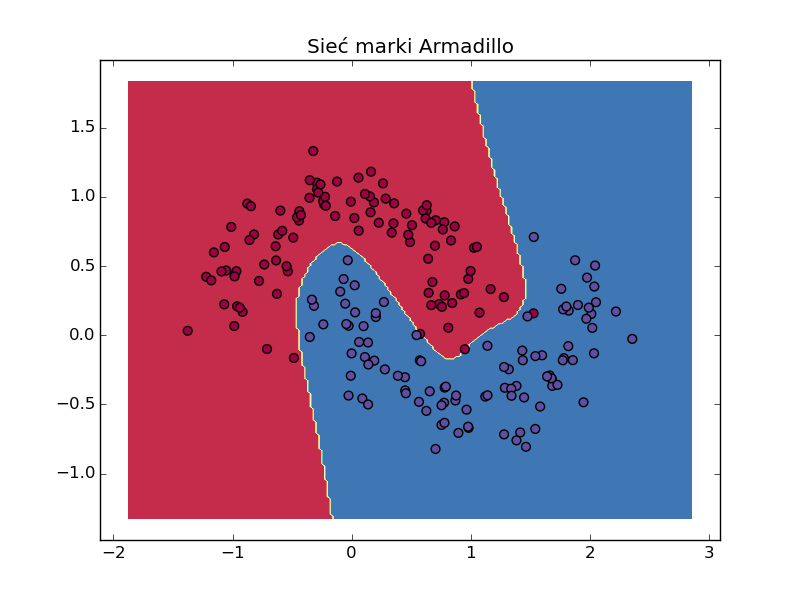
\includegraphics[width=0.50\textwidth]{figure_1.png}
	\caption{Political preferences - colors represent parties, points form the set T}
	\label{fig1}
\end{figure}


\paragraph{The solution}

How do we want to tackle that problem? We are going to use machine learning. First, we will come up with a function with some parameters and we will assume that this function can approximate the output we want to get, and using the training set we will try to find optimal values of the parameters - optimal in the sence that with them function gives the best approximation.

So, what will be our parametrized function? Let us summon a mathematical abstraction called neural network. Basic building block of a neural network is a perceptron - a function that takes a vector as an input and produces a single scalar as an output. Input of one perceptron can consist of outputs of other perceptrons - therefore perceptrons can be connected forming a directed graph called \emph{the net}. The net is usually aligned into layers - input layer, one or more hidden layers, and output layer, as shown in Figure \ref{fig2}. In such aligment, we can treat the whole \emph{layer} as a function that takes a matrix as an input and produces some other matrix as an output, and output of one layer becomes input of another. How does the perceptron - and therefore the layer compute output? Perceptron has a vector of weights $W$ a free term $b$, and an \emph{activation function} $s$. It takes input vector $x$, computes scalar product with $W$, adds the free term $b$, and passes that through the activation function. Generalizing, the \emph{layer} has a \emph{matrix} of weights $W$ and a \emph{vector} of free terms $b$ and the activation function. So, the formula for the output is the following:

\[ y = s(Wx + b) \]

In our case - the classification problem - the input will be $n$-dimensional vector of the point coordinates, and the output will be $k$-dimensional vector where the i-th element will be the probability that the point belongs to the i-th class.

\begin{figure}[fig2]
	
\label{fig:fig2}
  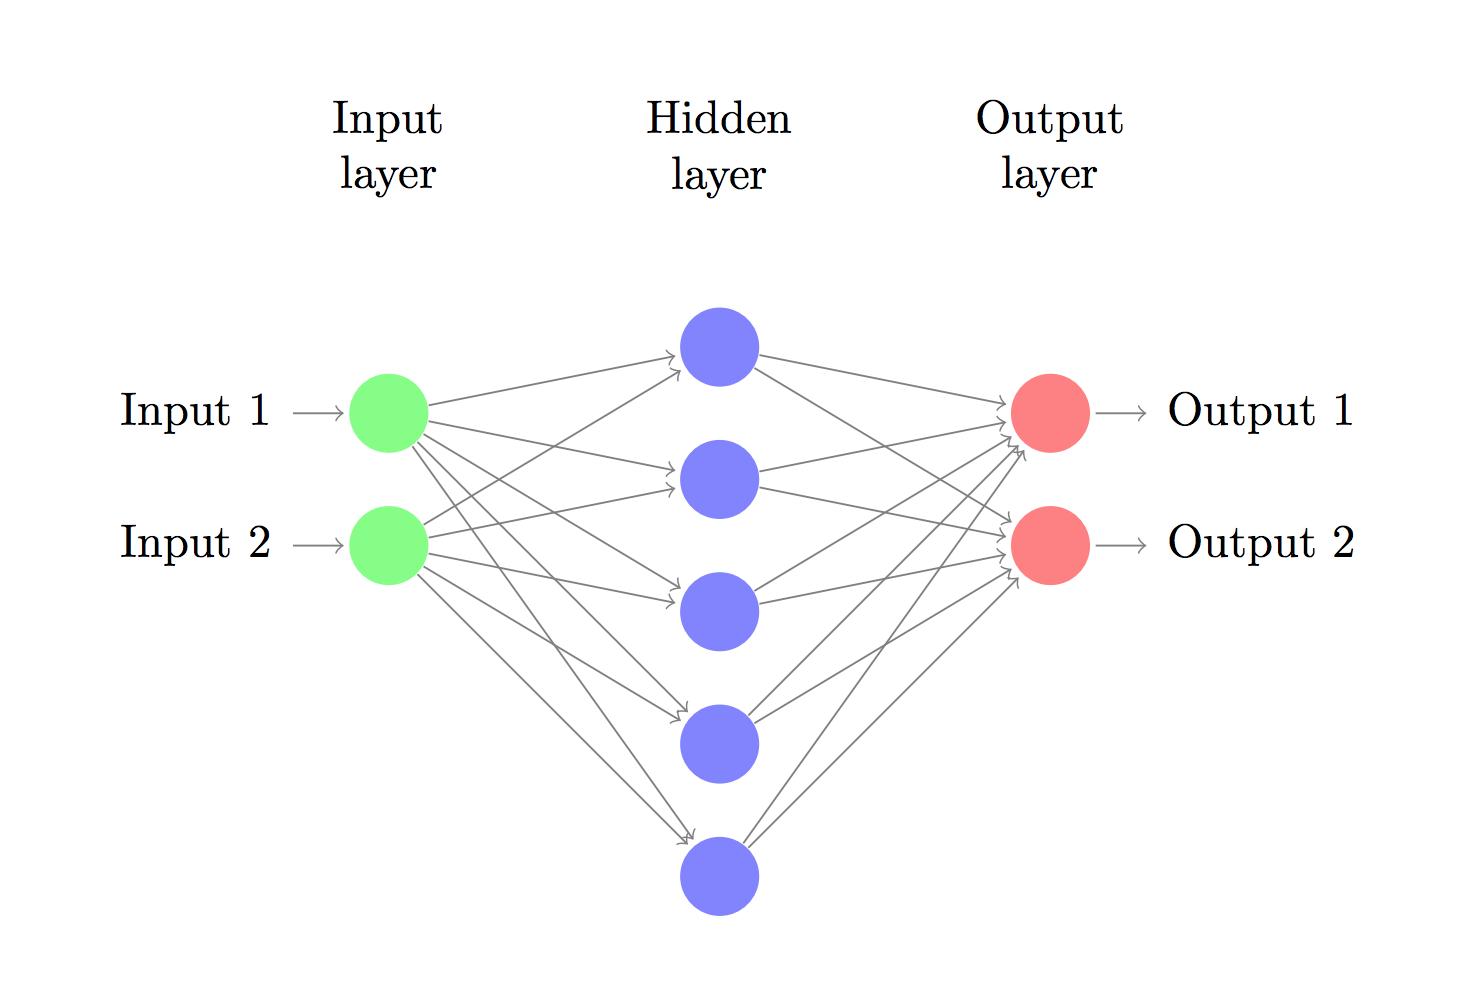
\includegraphics[width=0.60\textwidth]{network-schema.png}
	\caption{Schema of the neural network}
	\label{fig2}
\end{figure}

\paragraph{The implementation}

On of the advantages of the C++ language is its strong type system. It makes it much easier working with legacy code or with a library previously unknown to the programmer, because types alone can give a lot of information about what a given method or class is actually doing. We wanted to follow that path and we wanted our implementation to have types reflecting the mathematical model we described above. Armadillo provided us with classes for matrix and vector - \emph{mat} and \emph{rowvec}, what we have to do was to implement classes representing layer of the network and the whole network. (Actually we could also model perceptron as a separated class, but we decided not to do it as it would be too detalistic and would make things more complex and not more simple). Diagram of our classes with their interfaces can be seen on Figure \ref{fig:fig1}

\begin{figure}[fig2]
	
\label{fig:fig3}
  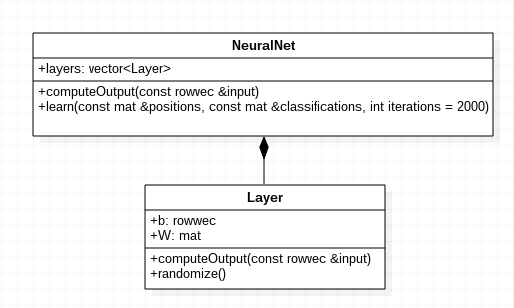
\includegraphics[width=0.60\textwidth]{uml-diagram.png}
	\caption{UML diagram of our implementation (library classes not shown)}
	\label{fig3}
\end{figure}


%\bibliography{mybibfile}

 \begin{thebibliography}{00}

% \bibitem must have the following form:
%   \bibitem{key}...
%

 \bibitem{armadillo} Armadillo homepage http://arma.sourceforge.net
 
 \bibitem{stack} Stack overflow

 \end{thebibliography}

\end{document}
